
\subsection{研究目标}
% 武旭同话术,待修改
基于上述研究进展,本研究面向社会-水文学研究前沿和黄河流域高质量发展的国家需求,以黄河流域为研究区,结合水文气象观测、社会经济统计、历史数据重建、遥感反演等获取多源数据,借助统计分析和模型模拟等手段,分析黄河流域人水关系的演变过程和驱动机制。具体研究目标如下:

(1)为“流域人水关系”提出概念定义与便于研究识别其演变规律的分析框架,进而分别在千年尺度和百年尺度上,定量划分黄河流域人水关系演变的主要阶段。
(2)结合多源数据的统计分析,利用因果推断方法和复杂系统的多主体建模,识别推动黄河流域人水关系变化的关键机制,定量评估其产生的影响。


\subsection{研究内容}

针对流域这个特定的人地关系地域系统(或社会-生态系统)给出“人水关系”的概念定义,为满足不同时间尺度的分析需要,建立流域系统层面的人水关系变化分析框架。在此框架的基础上,本研究具体包含以下主要内容:

% 开题报告
(1)黄河流域历史时期流域稳态演变:识别历史时期不断增强的人类活动压力超越气候周期变化的驱动力的时间,以及两者主导并推动黄河流域水沙特征突破临界点的稳态转换过程,分析该稳态转换发生之前黄河的人水关系状态。
% 接下来利用建立的分析框架对黄河流域历史上的大事记进行分析,梳理出黄河流域人-水关系演变的主要脉络。最后利用系统回顾法,整合近代有研究以来对黄河人-水关系变化的定量分析成果,建立黄河流域人-水关系变化数据库,综合分析有研究以来人-水系统的主要驱动因素及演化路径。 

(2)黄河流域近百年流域水治理演变:分析上世纪六十年代有实测数据以来,黄河流域“有多少水、怎么用水、怎么分水”如何随时间变化,以及三者如何共同体现流域水治理变化,并解释这些变化背后流域系统如何被人类活动所主导。

(3)黄河流域分水制度改革的影响:识别黄河流域在上世纪八十年代治理转型期间,先后于1987年和1998年两次改革流域水资源分配制度对流域系统的作用机制,分析其如何自上而下重塑社会-生态系统结构、以及对不同地区用水量的影响。

(4)黄河灌溉水分配的多主体建模:识别黄河流域在上世纪八十年代治理转型期间,流域用水的利益相关者对系统环境和制度变化的响应机制,分析其如何通过挑战水资源分配,自下而上地对流域转型做出适应,以及对水资源利用方式的影响。

基于上述研究内容,本研究的技术路线如图\ref{ch1:fig:workflow}所示:

\begin{figure}[htb] % use float package if you want it here
    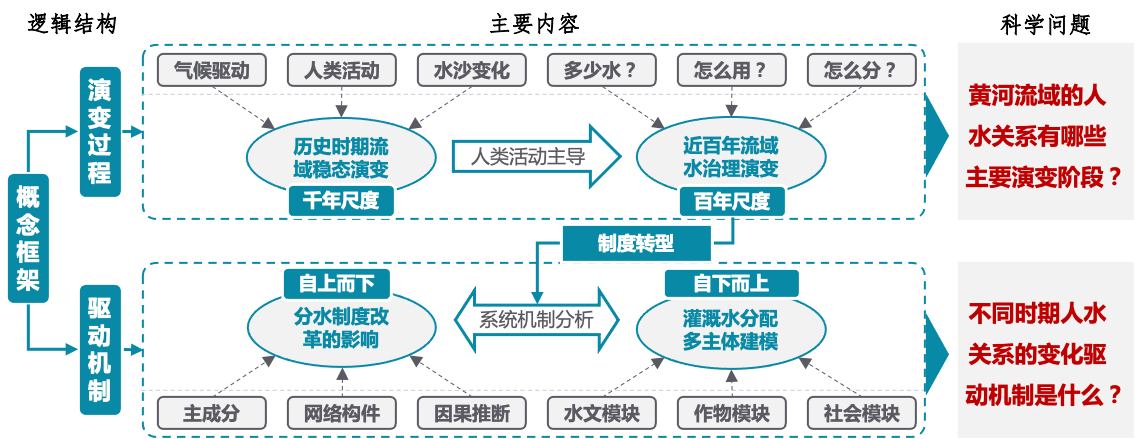
\includegraphics[width=\textwidth]{img/ch1/ch1_workflow.png}
    \caption{研究技术路线图}\label{ch1:fig:workflow}
\end{figure}

首先,发展流域系统人水关系演变的概念框架,明晰流域人水关系的概念内涵,厘定怎样的变化可以被识别为发生了“流域人水关系演变”,以及有哪些潜在的驱动机制会导致这类变化。
接下来利用研究概念框架,分别在千年尺度和百年尺度上识别流域人水关系的演变过程,两者主要差异除分析的时间尺度和精度不同外还有:
(1)千年尺度上,黄河流域的水沙特征发生从气候周期驱动向人类活动主导的过程,需要识别这一稳态转换的发生过程。
(2)百年尺度上,黄河流域的“自然-社会二元水循环”则已由人类活动主导,需要识别流域水治理系统发生稳态转换的过程。
通过整合千年尺度和百年尺度的人水关系演变,可以回答“黄河流域的人水关系有哪些主要演变阶段?”的科学问题,并总结各阶段黄河流域人水关系的系统特征。

在此基础上,针对百年尺度上由人类活动主导发生的制度转型期,以对黄河流域影响最为深远的水资源分配制度为例,分别从自上而下和自下而上两个路径分析流域系统的变化机制:
(1)自上而下:使用主成分分析、社会-生态系统网络构件识别、因果推断模型,分析制度改革对黄河流域系统结构及不同地区用水量的影响。
(2)自下而上:使用由水文模块、作物灌溉模块、社会模块构成的多主体模型,分析利益相关者众多的作物灌溉过程如何响应环境和制度变化,最终导致流域水资源利用模式的改变。
% % 帅王 2023
% (1)黄河流域人地系统结构特征及其时空演变
% 整合社会-生态要素及其相互作用关系构建人地系统网络结构图,利用网络分析方法刻画要素相互作用特征,发展网络指标量化人地系统结构特征并分析上中下游及过去四十年来的时空演变规律,识别其中关键社会-生态要素。
% (2)黄河流域社会-生态-水沙协同演变规律与耦合机理
% 系统研究黄河流域上游自然保护与生态恢复、中游退耕还林还草、下游水沙调控及湿地保育等综合措施对水沙和生态过程的影响,量化人地系统网络结构变化的效应,辨识水沙-社会经济-生态的协同演变规律。
% (3)黄河流域人地系统耦合模型
% 发展包含关键人类活动的生态水文过程模型,建立流域多主体模型,研究流域自然过程与社会经济过程的尺度匹配与转换方法,发展生态水文过程模型与多主体模型的耦合器,建立黄河流域人地系统耦合模型。
% (4)情景模拟与人地系统统筹优化
% 集成气候变化情景和人类活动情景,结合流域和政策情景构建黄河流域未来发展情景集,借助耦合模型模拟不同情景下流域社会-生态-水沙多过程协同演化趋势,探索流域协同治理的机制与路径。

\subsection{关键科学问题}

(1)黄河流域的人水关系有哪些主要演变阶段?

(2)不同时期人水关系变化的驱动机制是什么?
